\documentclass[a4paper,11pt]{report}

%%[inserting images of PostScript, JPEG, PNG and so on]
%% choose and comment-out the following packages
\usepackage{graphicx} % for \includegraphics[width=3cm]{sample.eps}
%\usepackage{epsfig} % for \psfig{file=sample.eps,width=3cm}
%%\usepackage{epsf} % for \epsfile{file=sample.eps,scale=0.6}
%\usepackage{epsbox} % for \epsfile{file=sample.eps,scale=0.6}

%% You may use dvipdfm for directly creating PDF from DVI.
%\usepackage[dvipdfm]{color,graphicx}
%% bookmarking with dvipdfm
%\usepackage[dvipdfm,bookmarks=true,bookmarksnumbered=true,bookmarkstype=toc]{hyperref}

%\usepackage{times} % use Times Font instead of Computer Modern

\setcounter{tocdepth}{3}
\setcounter{page}{-1}

\setlength{\oddsidemargin}{0.1in}
\setlength{\evensidemargin}{0.1in} 
\setlength{\topmargin}{0in}
\setlength{\textwidth}{6in} 
%\setlength{\textheight}{10.1in}
\setlength{\parskip}{0em}
\setlength{\topsep}{0em}

%\newcommand{\fig}[1]{{\bf Fig.\ref{#1}}}

%% [IMPORTANT] package for title generation (english version)
\usepackage{sie-en}

%% title of thesis
%% DON'T PUT \\ AT THE END OF THE TITLE. IT CAUSES ERROR!!
\title{Visualization of Viewing Fields of Surveillance Cameras by Using Mixed Reality}
%% name of author
\author{Dao Ngoc Thanh}
%% name of advisor
\advisor{Yuichi Ohta}

%% major and degree and date (chooose one)
%% [NOTICE] Month varies with majors. (submitted date)
%\majorfield{Policy and Planning Science} \degree{Economics} \yearandmonth{January 2002}
%\majorfield{Policy and Planning Science} \degree{Policy and Planning Sciences} \yearandmonth{January 2002}
%\majorfield{Policy and Planning Science} \degree{Engineering} \yearandmonth{January 2002}
%\majorfield{Quantitative Finance and Management} \degree{Finance} \yearandmonth{January 2002}
%\majorfield{Quantitative Finance and Management} \degree{Management} \yearandmonth{January 2002}
%\majorfield{Quantitative Finance and Management} \degree{Policy and Planning Sciences} \yearandmonth{January 2002}
%\majorfield{Computer Science} \degree{Engineering} \yearandmonth{February 2002}
%\majorfield{Advanced Engineering Systems} \degree{Engineering} \yearandmonth{February 2002}
%\majorfield{Engineering Mechanics and Energy} \degree{Engineering} \yearandmonth{February 2002}
%\majorfield{Risk Engineering} \degree{Engineering} \yearandmonth{2002}
%\majorfield{Risk Engineering} \degree{Policy and Planning Sciences} \yearandmonth{2002}

\majorfield{Intelligent Interaction Technologies} \degree{Engineering} \yearandmonth{March 2009}

\begin{document}
\maketitle
\thispagestyle{empty}
\newpage

\thispagestyle{empty}
\vspace*{20pt plus 1fil}
%\parindent=1zw
\noindent
%%
%% Abstract
%%
\begin{center}
{\bf Abstract}
\vspace{5mm}
\end{center}
This research lies in the domain of Outdoor Mixed Reality. It aims to visualize the viewing fields of outdoor surveillance cameras on the screen of mobile devices. In an outdoor environment where cameras on mobile devices can be used, it is required that users can easily understand the visualized viewing fields of surrounding surveillance cameras. Moreover, the visualization system must provide realtime video with no human-sensible delay.

In this research, we study five visualization methods and propose a prototype system based on server-side PTAM. The prototype requires no GPS or gyrocompass devices. We have implemented the prototype and conducted some experiments in our campus.

%%%%%
\par
\vspace{0pt plus 1fil}
\newpage

\pagenumbering{roman} % I, II, III, IV 
\tableofcontents
\listoffigures
%\listoftables

\pagebreak \setcounter{page}{1}
\pagenumbering{arabic} % 1,2,3

\chapter{Introduction} % Write in your own chapter title
\label{Chapter1}
\lhead{Chapter 1. \emph{Introduction}} % Write in your own chapter title to set the page header

%------------------------------------------------------------------------------

\section{Introduction}

Surveillance cameras have become popular and placed almost everywhere, e.g. train stations, airports, banks, shops, streets. The balance between security and privacy is an active subject for political/social debates. It is hard to keep a balance between security and privacy, a person may feel protected when he knows himself and his surroundings are being observed, but at the same time he may feel uncomfortable.

The information that a person probably wants to know most about surveillance cameras is probably their viewing fields, e.g. where the cameras are, whether he is inside the observed area. For indoor environment, because the space is usually small, people may easily locate the position and estimate the viewing fields of the cameras. For outdoor environment, it is almost impossible to find surveillance camera systems which support people to visually know the viewing fields in real scene. Fortunately, there is a technology which can be applied for situations like this: MR (Mixed Reality). MR is the encompassing of both Augmented Reality and Augmented Virtuality, merging the real world in which we are living and the virtual world created by computers. MR produces new environments where real and virtual entities can co-exist and interact in realtime \citep{Reference3}.

MR applications are traditionally equipped with HMDs (Head Mounted Display) as shown in figure \ref{fig:HMD}. However, HMDs are usually bulky and inconvenient for outdoor applications, where wide-range mobility is crucial. In recent years, mobile devices have become popular, devices like cell phones, PDA (Personal Digital Assistants) can be seen everywhere. Their prices have come down and they could reach the hands of common people even in developing countries like Viet Nam. High-end mobile devices, such as Apple iPhone and Google T-Mobile G1, usually have high specifications. More importantly for outdoor MR applications, they are almost always equipped with built-in cameras, GPS (Global Positioning System), and accelerometer devices. These auxiliary devices usually meet the need of common outdoor MR applications because they provide video and information to help estimating position and orientation of the mobile devices \citep{Reference2} \citep{Reference4}.

\begin{figure}[htbp]
	\centering
	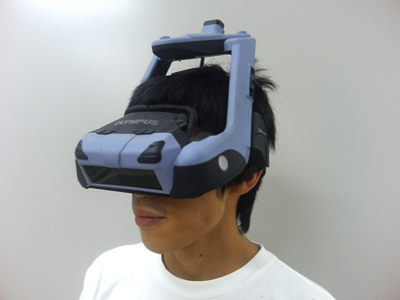
\includegraphics{./Primitives/hmd.jpg}
	\rule{35em}{0.5pt}
	\caption[An HMD]{An HMD}
	\label{fig:HMD}
\end{figure}

However, image processing applications usually need large memory and powerful computing capability. Even current high-end cell phones and PDAs may not run MR applications properly without special program optimizations. For compute-intensive outdoor MR applications, more powerful UMPCs (Ultra-Mobile Portable Computer) like the one in figure \ref{fig:VAIO} may be used. UMPCs equipped with built-in camera, GPS, and gyrocompass devices have been found practical and are a topic of many researches \citep{Reference2} \citep{Reference4} \citep{Reference13}.

\begin{figure}[htbp]
	\centering
	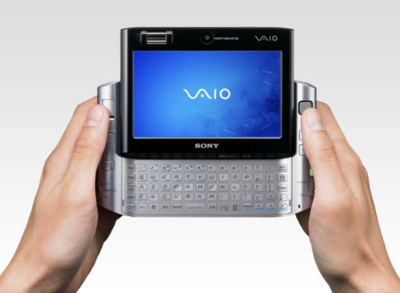
\includegraphics{./Primitives/vaio.png}
	\rule{35em}{0.5pt}
	\caption[Sony VAIO VGN-UX90PS with a camera at the front]{Sony VAIO VGN-UX90PS with a camera at the front (top, center)}
	\label{fig:VAIO}
\end{figure}

\begin{figure}[htbp]
	\centering
	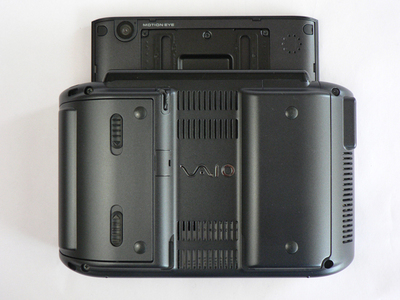
\includegraphics{./Primitives/vaio_back.jpg}
	\rule{35em}{0.5pt}
	\caption[Sony VAIO VGN-UX90PS with a camera at the back]{Sony VAIO VGN-UX90PS with a camera at the back (top, left)}
	\label{fig:VAIOBack}
\end{figure}

This research aims to visualize the viewing fields of outdoor surveillance cameras on the screen of mobile devices. In this research, we propose:

\begin{itemize}
	\item Five methods to visualize viewing fields of surveillance cameras for outdoor MR (chapter \ref{Chapter2}).
	\item A prototype based on server-side PTAM (Parallel Tracking and Mapping) \citep{Reference12} technology (chapter \ref{Chapter3}). The prototype uses a Sony VAIO VGN-UX90PS (appendix \ref{AppendixA}) and provides realtime video. Because the VAIO is still weak to do PTAM processing, we connect it wirelessly to an Apple MacBook Pro, which actually does the heavy work of PTAM. This results in a prototype providing realtime video with no requirement for any GPS or gyrocompass devices.
\end{itemize}

An experiment using the prototype to evaluate the visualization methods is described in chapter \ref{Chapter4}.

%------------------------------------------------------------------------------

\section{Use Cases}
\label{UseCases}

Using the prototype we make in chapter \ref{Chapter3}, when a user wants to see the visualized viewing fields of surrounding surveillance cameras on his own mobile device screen, the typical usage scenario is (figure \ref{fig:VAIOMacBookPro}):

\begin{enumerate}
	\item The user points the mobile camera in a certain direction.
	\item Through wireless network, the mobile device continuously sends frames captured by the camera of the scene to a more powerful remote computer for processing.
	\item Based on the frames, the remote computer estimates the position and orientation of the mobile camera, and send them to the mobile device.
	\item Based on the position and orientation data, the mobile device correctly renders virtual CG (computer graphics) objects onto the frames to visualize viewing fields of the surrounding surveillance cameras, and renders the frames onto its screen.
\end{enumerate}

\begin{figure}[htbp]
	\centering
	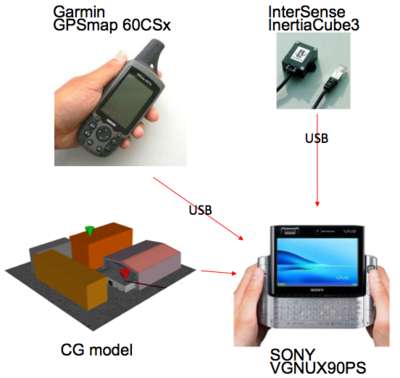
\includegraphics{./Figures/vaio_macbookpro.png}
	\rule{35em}{0.5pt}
	\caption[Prototype architecture]{Prototype architecture}
	\label{fig:VAIOMacBookPro}
\end{figure}

When the user changes the position or orientation of the mobile camera, the video displayed on the screen will simultaneously change accordingly to the camera movement.

The purpose of the above use case is to give an example of the application of visualizing viewing fields of surveillance cameras and to give a rough idea of how the prototype works. There may be other applications. For example, we can build a system which visualizes ``safe paths'' or ``safe areas'' for pupils (figure \ref{fig:HomeSchool}). Pupils can use their cell phones to see if their current location is being well observed when they walk to school or go home from school.

\begin{figure}[htbp]
	\centering
	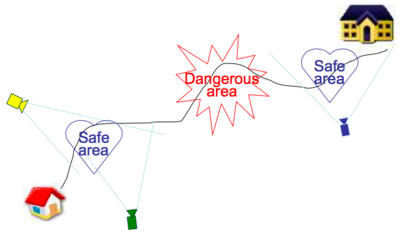
\includegraphics{./Primitives/home_school.png}
	\rule{35em}{0.5pt}
	\caption[Safe path to school]{Safe path to school}
	\label{fig:HomeSchool}
\end{figure}

%------------------------------------------------------------------------------

\section{Background}

For outdoor MR, bulky devices or devices that reduce the mobility of users are not preferable. For example: big computers, devices wired to a fixed position, devices with big auxiliaries, big HMDs, HMDs that prevent users from seeing the outdoor environment while walking\ldots As a result, devices for outdoor MR should be small, lightweight, should connect wirelessly to other devices if they need to.

MR programs usually need to know the position and orientation of the devices in order to merge images of the virtual world to the correct place of the images of the real world. For indoor environment, marker-based solutions are known to work very well \citep{Reference20}. However, outdoor environment is usually large thus it is impossible to put markers everywhere. There have been many researches that use UMPCs equipped with GPS and/or gyrocompass devices \citep{Reference2} \citep{Reference4} \citep{Reference13}. Hardware devices have been becoming smaller and more powerful according to Moore's law. Today's high-end cell phones, like Apple iPhone and Google T-Mobile G1, usually have built-in GPS and accelerometer devices. Because of their small size, high specifications, and competitive prices, such devices have found their use in outdoor MR applications and researches, like \htmladdnormallink{Sekai camera}{http://sekaicamera.com/} \citep{Reference18} and \htmladdnormallink{Enkin}{http://www.enkin.net/} \citep{Reference19}.

However, normal GPS devices have error of about 5--10 m, and gyrocompass devices suffer from drift error. There have been many researches that are based on the images taken by the camera on the mobile device to deal with this problem. We can follow the approach that uses gravity accelerometer to help eliminate drift error, model-based tracking with edge and texture tracker to help produce accurate localization result \citep{Reference13}. There is also an extreme approach that completely does not require GPS or gyrocompass devices, only uses the images taken by the camera and a landmark database of natural feature points built before-hand \citep{Reference21}.

When MR programs need more memory or CPU power than the mobile devices can provide to run, we have a backup solution in which the mobile devices connect wirelessly to remote non-mobile computers to ask for help. It is possible send realtime video images wirelessly to remote computers for processing because wireless network speed may go up to 54 Mbps. This may be a good approach because Moore's law has slowed down in recent years, thus we cannot expect the specifications of mobile devices to go much higher anytime soon while at the same time keeping their mobility.

\chapter{Background}
\label{Chapter2}
\lhead{Chapter 2. \emph{Background}}

\chapter{Visualization Methods}
\label{Chapter3}
\lhead{Chapter 3. \emph{Visualization Methods}}

\section{Viewing Volume, Viewing Frustum, Viewing Field, and Visualization Requirements}
\label{VisualizationRequirements}

In natural sense, viewing volume of a camera is defined by an infinite half cone, apex of which corresponds to the focal point of the camera. Because real computers cannot have unlimited resources, in practical computer 3D technology we usually limit the bottom of the cone by a far clip plane, then limit the top of the cone even more by a near clip plane, and express the result by a frustum, as illustrated in figure \ref{fig:ViewingVolume}. To visualize the viewing volume, there may be many methods other than directly rendering the volume. Thus in this research we abstract the viewing volume by the term ``viewing field".

\begin{figure}[htbp]
	\centering
	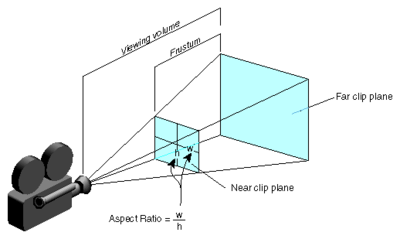
\includegraphics{./Primitives/viewing_volume.png}
	\rule{35em}{0.5pt}
	\caption[Viewing volume of camera]{Viewing volume of camera}
	\label{fig:ViewingVolume}
\end{figure}

There may be many visualization methods, not limited to the ones discussed in the next section. But for a method to find practical use in outdoor MR, it should be able to be implemented (see section \ref{AUseCase} to have a rough illustration) so that it meets the following basic qualitative requirements, expressed in the ``it should" tongue of most DSLs (Domain Specific Language) of the BDD (Behavior Driven Development) methodology in software engineering:

\begin{itemize}
	\item It should be easy for the user to understand when they see the visualized viewing fields of surrounding surveillance cameras.
	\item It should work in realtime. When the user changes the position or orientation of the mobile device, the video displayed on the screen of the mobile device should simultaneously change accordingly to the movement without much delay.
	\item It should have good accuracy. In order to correctly overlay CG objects onto the original video, the position and orientation of the mobile device's camera must be estimated within a small error.
	\item It should be robust to disturbance in outdoor environment. In outdoor environment, naturally there may be many passers-by and they may prevent the mobile device's camera from continuously capturing a scene. If the system use GPS device, the GPS signal strength may change a lot when the user walk from an open space to a space shadowed by trees or buildings.
\end{itemize}

When implementing the prototype in chapter \ref{Chapter4} and conducting experiment to evaluate the visualization methods, we must take the above requirements into account.

\section{Visualization Methods}
\label{VisualizationMethods}

In this section, we propose five methods to visualize viewing fields of . This section discusses the idea and algorithm of the methods. Based on this discussion, chapter \ref{Chapter4} will implement and integrate these methods into a working prototype.

\subsection{Volume Method}

As discussed above, the natural method to visualize the viewing field is thus simply visualizing this volume as shown in figure \ref{fig:VolumeMethod}. However, the volume usually occupies all the scene viewed from the mobile camera, especially if the user is inside the viewing volume. The visualization produced by this method is hard to understand.

\begin{figure}[htbp]
	\centering
	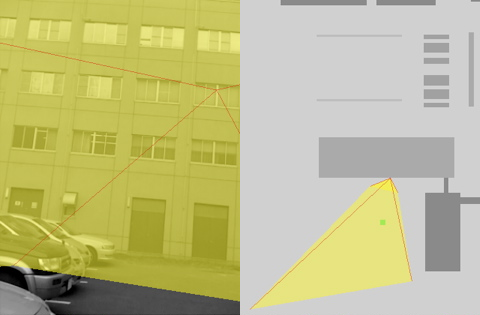
\includegraphics{./Primitives/theory_volume.png}
	\rule{35em}{0.5pt}
	\caption[Volume Method]{Volume Method}
	\label{fig:VolumeMethod}
\end{figure}

\subsection{Shadow Method}

The fact that the image captured by the camera is perspective projection of the volume into the near plane of the frustum gives us another method. This method visualizes the virtual shadow created by the light positioned at the eye-point of the camera and the near plane of the frustum, as shown in figure \ref{fig:ShadowMethod}. This method gives more understandable visualization. There are various ways to render the shadow, the two popular ones are shadow mapping \citep{Reference7} \citep{Reference8} and volume shadow \citep{Reference9}.

\begin{figure}[htbp]
	\centering
	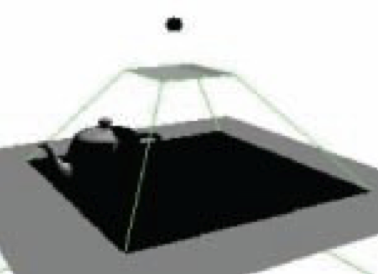
\includegraphics{./Primitives/theory_shadow.png}
	\rule{35em}{0.5pt}
	\caption[Volume Method]{Shadow Method}
	\label{fig:ShadowMethod}
\end{figure}

\subsection{Contour Method}

An alternative method is to only visualize the contours of the shadow, as shown in figure \ref{fig:ContourMethod}. Rendering only the contour is much lighter than rendering the whole shadow, thus this method is supposed to be much faster.

\begin{figure}[htbp]
	\centering
	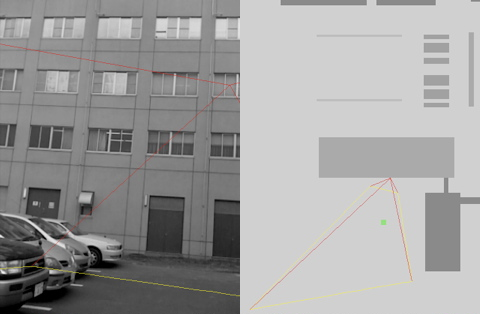
\includegraphics{./Primitives/theory_contour.png}
	\rule{35em}{0.5pt}
	\caption[Volume Method]{Contour Method}
	\label{fig:ContourMethod}
\end{figure}

\subsection{Vector Method}

For most of the time, a person may want to know not only the viewing field, but also the position and distance to the surveillance camera, To visualize this information, we propose a method using vectors as shown in figure \ref{fig:VectorMethod}. In the figure, all the vectors are pointing the camera, and the length of the vectors are reverse proportional to the distance from the root of the vectors to the camera.

\begin{figure}[htbp]
	\centering
	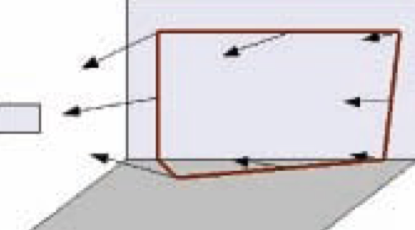
\includegraphics{./Primitives/theory_vector.png}
	\rule{35em}{0.5pt}
	\caption[Volume Method]{Vector Method}
	\label{fig:VectorMethod}
\end{figure}

\subsection{Animation Method}

We are studying the visualization method in which animate objects coming from the surveillance cameras are used to visualize the viewing fields. This method has  many advantages:

\begin{itemize}
	\item The moving objects start form the surveillance camera positions, as a result the user easily knows the camera positions.
	\item Event when the mobile camera is fixed at a certain position and orientation, the visualization effect is still achieved.
	\item The moving objects do not block the scene, as a result the user can see the scene and visualized camera viewing fields at the same time.
\end{itemize}

\begin{figure}[htbp]
	\centering
	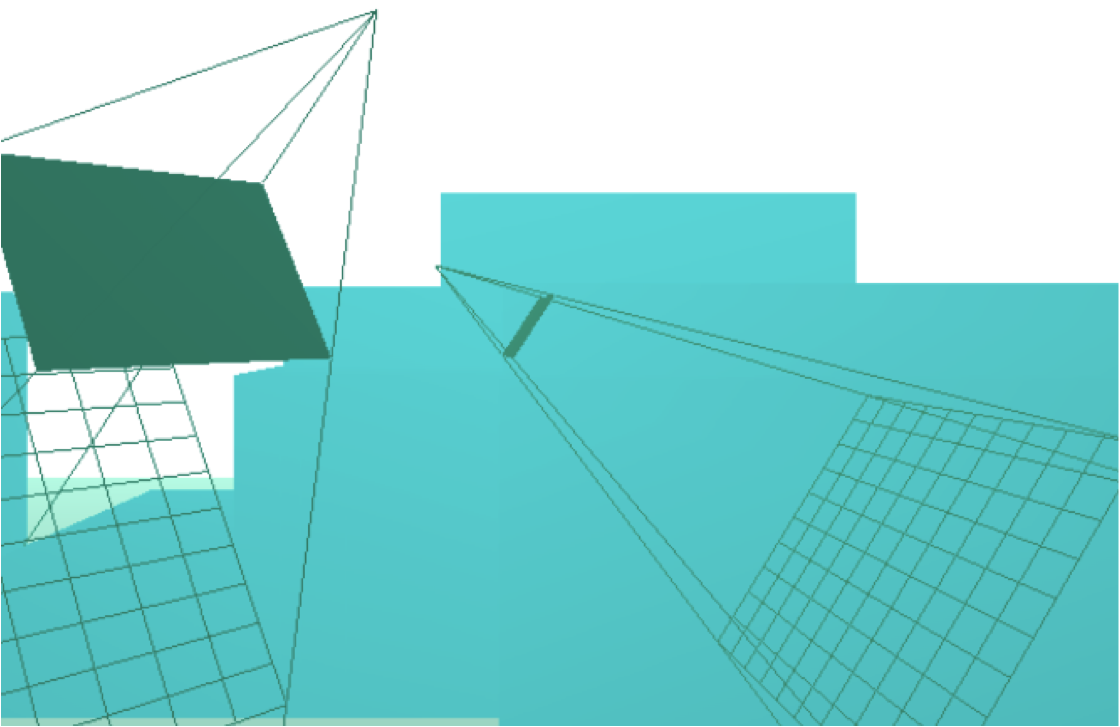
\includegraphics{./Primitives/theory_animation.png}
	\rule{35em}{0.5pt}
	\caption[Volume Method]{Animation Method}
	\label{fig:AnimationMethod}
\end{figure}

\chapter{Prototype System Implementation}
\label{Chapter4}
\lhead{Chapter 4. \emph{Prototype System Implementation}}

This chapter describes a prototype implementation of the visualization methods in chapter \ref{Chapter3}.

mobile device is equipped with a camera, GPS and gyrocompass devices. The camera lets the user take video from his own point of view. GPS and gyrocompass devices give the system the position and orientation of the mobile camera, respectively.


\section{System Architecture}

\subsection{Hardware}

\begin{itemize}
	\item The mobile device used is a SONY VAIO VGN-UX90PS, its specifications is in appendix \ref{AppendixA}. It has two built-in cameras. We use only the camera at the back as shown in figure \ref{fig:VAIOBack}, at 15fps@640x480.
	\item The gyrocompass attached is an InterSense InertiaCube3. It is one of the world's smallest inertial orientation reference system, its specifications is in appendix \ref{AppendixB}. The update rate is 180Hz, which eliminates tracker induced lag. It is connected to the mobile device with and RS322-USB adapter.
	\item The RTK-GPS system is shown in Figure [cite]. It is also connected to the mobile device with and RS232-USB adapter.
\end{itemize}

\subsection{Software}

The system does not use a server or any real surveillance camera. In place of those, 3D model of the building of the College of International Studies and the gymnasium (Figure [cite]), together with the hard coded geometry information about the virtual surveillance cameras are used.

The best visualization method is expected to be found visually and practically. A good visualization method can be the combination of many others at any extent. Thus, trial and error methodology can be applied here. To shorten the trial and error cycles, a good developmental environment of the preliminary system in this research, C language and OpenGL API \citep{Reference10} were used at first. Because both the language and the API are in too low level, the development speed was slow. Later, C language was replaced by Ruby language. The development speed was better but still slow. As as a result, it was concluded that the speed of the development is largely affected by the API rather than the language. Consequently, a higher level API has been adopted: OGRE \citep{Reference11}. OGRE, Object-Oriented Graphics Rendering Engine, is a scene-oriented, flexible 3D rendering engine written in C++ designed to make it easier and more intuitive for developers to produce applications utilizing hardware-accelerated 3D graphics. The class library abstracts all the details of using the underlying system libraries like Direct3D and OpenGL and provides an interface based on world objects and other intuitive classes.

\section{Viewing Modes}

\section{System Characteristics}

Largely because the part to retrieve video images from the mobile camera is blocking, i.e. other parts of the program must wait while the images are being retrieved, the program is designed to be multithreaded. Its structure is shown in Figure [cite]. Visualization methods are programmed as visualizer plugins, so that the currently selected visualization method is changed by simply changing its corresponding plugin to another one. The thread to retrieve the image from the mobile camera runs at about 12fps@320x240, while the thread to display the final output image runs at about 10fps@640x480. This allows farther complex computation to be applied without noticeable delay and decrease in frame rates.

\chapter{Conclusion and Future Directions}
\label{Chapter5}
\lhead{Chapter 5. \emph{Conclusion and Future Directions}}

In this research, we have proposed an outdoor MR system which enables a user to easily use his mobile device to have a visualization of viewing fields of surveillance cameras surrounding himself in realtime.

* server side: multicore
* client side:
	* Actually, processing work on the VAIO is light (send image, display ...)=> tweak to run on lower spec mobile devices like Apple iPhone, Google T-Mobile G1.
	* 5 years
* multi-sensor fusion


In the contrary, at this time the above devices are limited in memory and computing power because of their small size, thus usually not very suitable for MR applications (and image processing applications, in general), which usually need large memory and powerful computing capability.

=> 5 years

thuong co san ca gps va accelerator => sensor fusion

Moore's Law is the observation that the amount you can do on a single chip doubles every two years. But Moore's Law is taking a detour. Rather than producing faster and faster processors, companies such as Intel and AMD are producing multi-core devices: single chips containing two, four, or more processors. If your programs aren't concurrent, they'll only run on a single processor at a time. Your users will think that your code is slow.

Erlang is a programming language designed for building highly parallel, distributed, fault-tolerant systems. It has been used commercially for many years to build massive fault-tolerated systems that run for years with minimal failures.

Erlang programs run seamlessly on multi-core computers: this means your Erlang program should run a lot faster on a 4 core processor than on a single core processor, all without you having to change a line of code.

Erlang combines ideas from the world of functional programming with techniques for building fault-tolerant systems to make a powerful language for building the massively parallel, networked applications of the future.

This book presents Erlang and functional programming in the familiar Pragmatic style. And it's written by Joe Armstrong, one of the creators of Erlang.


Future directions:
* Co 2 huong: 1 la xu li tren 1 cai luon k can server => (One-)hand held mobile device co hardware spec ngay cang lon.
* 1 la dung server, nhung communication network phai nhanh => Cai iPhone gi do (nho cite) co the len den 45FPS! Mang cung nhanh <---

Moore's laws bi limit roi => vs. Tien the noi ve xu huong multicore CPU => van de server k phai lo nhieu!
Nho cite nhieu nhieu, cai thesis Erlang cua ong gi nhi?


\chapter*{Acknowledgements}
\addcontentsline{toc}{chapter}{\numberline{}Acknowledgements}

There are many people and organizations I would like to thank, without my study and this research would not have been possible.

I would like to thank professor Yuichi Ohta, associate professor Yoshinari Kameda, and associate professor Itaru Kitahara of the Computer Vision and Image Media Laboratory for their guidance on the field of computer vision and image processing, their support, comments, and valuable advices in the three years on this research. I would like to thank Shinya Yamazaki, Masayuki Hayashi, and other members of the laboratory for their help and discussion.

I would like to thank the Japanese Ministry of Education which has given me the chance to come to Japan and provided me with financial support in the early years. I would like to thank Watanuki International Scholarship Foundation, and Epson International Scholarship Foundation for their generous financial support in the last two years.

I would like to thank my family and friends in Viet Nam and friends in Tokyo, Takamatsu, and Tsukuba for their time, support and encouragement.

\newpage

\appendix % Cue to tell LaTeX that the following 'chapters' are Appendices

\chapter{Sony VAIO VGN-UX90PS}
\label{AppendixVAIO}

See figure \ref{fig:VAIO}.

\begin{itemize}
	\item Size: 150.2 x 95 x 32.2 mm
	\item Weight: 520 g
	\item CPU: Core solo U1400 1.20 GHz
	\item RAM: 512 MB DDR2
	\item OS: Microsoft Windows XP Professional (SP2)
	\item LCD Display: 4.5 inch wide TFT color LCD
	\item Display mode: 16190000 colors
	\item Video memory: 128 MB
	\item Interface:
		\begin{itemize}
			\item Hi-speed USB (USB 2.0)
			\item Network (LAN) connector
			\item Wireless IEEE801.11a/b/g, WPA2. Wi-Fi. Bluethooth2.0
		\end{itemize}
	\item Camera: Web camera MOTION EYE x 2
		\begin{itemize}
			\item 1/8 inch VGA Progressive CMOS, 3.3 M pixel, f = 2.6 mm F4
			\item 1/4 inch SXGA Progressive CMOS, 13.4 M pixel, f = 3.8 mm F4
		\end{itemize}
\end{itemize}

\chapter{Apple iPhone 3G}
\label{AppendixiPhone}

\begin{figure}[htbp]
  \centering
    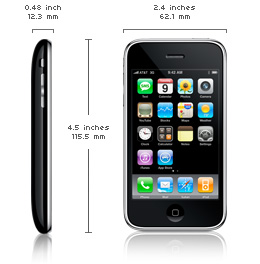
\includegraphics{./Primitives/iphone.jpg}
    \rule{35em}{0.5pt}
  \caption[Apple iPhone 3G]{The Apple iPhone 3G used in preliminary experiment}
\end{figure}

\begin{itemize}
	\item CPU: 620 MHz ARM
	\item GPU: PowerVR MBX Lite 3D
	\item Memory: 128 MB DRAM
	\item Display: 320 x 480
	\item Wi-Fi: 802.11b/g
	\item Assisted GPS, Accelerometer
	\item Battery: Up to 6 hours on Wi-Fi
	\item Capacity: 8 GB (flash memory)
\end{itemize}

\chapter{Apple MacBook Pro}
\label{AppendixMacBook}

\begin{figure}[htbp]
  \centering
    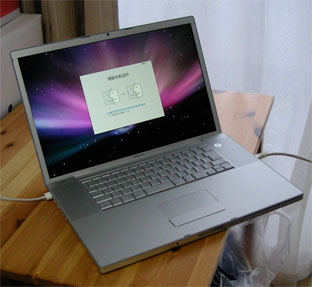
\includegraphics{./Primitives/macbookpro.jpg}
    \rule{35em}{0.5pt}
  \caption[Apple MacBook Pro]{The Apple MacBook Pro used in the prototype system}
\end{figure}

\begin{itemize}
	\item CPU: Intel Core 2 Duo (Number Of Cores: 2) 2.4 GHz, L2 Cache: 3 MB
	\item Memory: 2 GB 667 MHz DDR2 SDRAM
	\item Bus Speed: 800 MHz
	\item OS: Mac OS X 10.5.6, Microsoft Windows XP Professional SP2
\end{itemize}

\chapter{Garmin GPSmap 60CSx}
\label{AppendixGPS}

\begin{figure}[htbp]
  \centering
    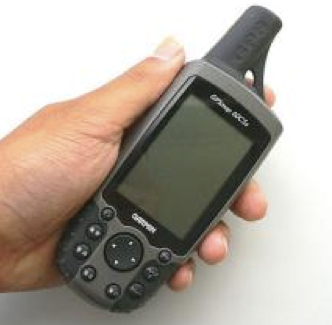
\includegraphics{./Primitives/gpsmap60csx.png}
    \rule{35em}{0.5pt}
  \caption[Garmin GPSmap 60CSx]{Garmin GPSmap 60CSx}
\end{figure}

\begin{itemize}
	\item Electronic compass feature:
		\begin{itemize}
			\item Accuracy: 2 degrees with proper calibration (typical); 5 degrees extreme northern and southern latitudes 
			\item Altimeter feature: (GPSMAP 60CSx only) 
			\item Resolution: 1 foot 
			\item Range: -2,000 to 30,000 feet 
			\item Elevation computer: Current elevation, resettable minimum and maximum elevation, ascent/descent rate, total ascent/descent, average and maximum ascent/descent rate 
			\item Pressure: Local pressure (mbar/inches HG) 
		\end{itemize}
	\item Physical:
		\begin{itemize}
			\item Size: 2.4W x 6.1H x 1.3D inches (61 x 155 x 33 mm) 
			\item Weight: 7.5 oz. (213 g) est. 
			\item Display: 1.5 x 2.2 inches (38.1 x 56 mm) 256-color transflective TFT (160 x 240 pixels) (160 x 240 pixels) 
  		\end{itemize}
	\item Navigation features:
		\begin{itemize}
			\item Waypoints/icons: 1000 with name and graphic symbol, 10 nearest (automatic), 10 proximity 
			\item Routes: 50 reversible routes with up to 250 points each, plus MOB and TracBack® modes 
			\item Tracks: 10K point automatic track log; 20 saved tracks 500 points each let you retrace your path in both directions
			\item Trip computer: Current speed, average speed, resettable max. speed, trip timer and trip distance 
			\item Map datums: More than 100 plus user datum 
			\item Position format: Lat/Lon, UTM/UPS, Maidenhead, MGRS, 
			\item Loran TDs and other grids, including user UTM grid only 
		\end{itemize}
	\item GPS performance 
		\begin{itemize}
			\item Receiver: 12 channel SiRFstar III (TM) high-sensitivity 
			\item GPS receiver (WAAS-enabled) continuously tracks and uses up to 12 satellites to compute and update your position 
			\item Acquisition times: Warm: $<$ 1 sec; Cold: $<$ 38 sec; AutoLocateTM: $<$ 45 sec 
			\item Update rate: 1/second, continuous 
			\item GPS accuracy: Position: $<$ 10 meters, typical; Velocity: .05 meter/sec steady state 
			\item DGPS (WAAS) accuracy: Position: $<$ 5 meters, typical; Velocity: .05 meter/sec steady state 
			\item Protocol messages: NMEA 0183 output protocol 
			\item Antenna: Built-in quad helix receiving antenna, with external antenna connection (MCX)
		\end{itemize}
\end{itemize}

\chapter{InterSense InertiaCube3}
\label{AppendixGyro}

\begin{figure}[htbp]
  \centering
    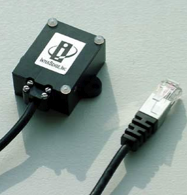
\includegraphics{./Primitives/inertiacube3.png}
    \rule{35em}{0.5pt}
  \caption[InterSense InertiaCube3]{InterSense InertiaCube3}
\end{figure}

\begin{itemize}
	\item Degrees of Freedom: 3 (Yaw, Pitch and Roll) 
	\item Angular Range Full: 360$^\circ$ - All Axes 
	\item Maximum Angular Rate: 1200$^\circ$ per second 
	\item Minimum Angular Rate: 0$^\circ$ per second 
	\item RMS Accuracy: 1° in yaw, 0.25$^\circ$ in pitch and roll at 25 $^\circ$C 
	\item RMS Angular Resolution: 0.03$^\circ$
	\item Serial Interface Update Rate: 180 Hz
	\item Minimum Latency: 2 ms for RS-232 (PC host OS dependent) 
	\item Prediction: up to 50 ms 
	\item Serial Rate: 115.2 kbaud 
	\item Interface: RS-232 Serial (shown above) 
	\item Size: (without mounting plate) 1.031 in x 1.544 in x 0.581 in (26.2 mm x 39.2 mm x 14.8 mm) 
	\item Weight: 0.6 ounces (17.0 g) 
	\item Cable Length: 15 ft. (4.572 m) - Max. 75 ft (22.86 m) 
	\item Power: 6 VDC, 40 ma 
	\item Operating Temperature Range: 0 to 70 $^\circ$C 
\end{itemize}


%% Bibliography
\addcontentsline{toc}{chapter}{\numberline{}Bibliography}
\renewcommand{\bibname}{Bibliography}
% use bibtex
\bibliographystyle{unsrt}
%\bibliography{samplebib}
%% [compile] bibtex sample-en; platex sample-en; platex sample-en;

%\bibliographystyle{unsrtnat}  % Use the "unsrtnat" BibTeX style for formatting the Bibliography
\bibliography{Bibliography}  % The references (bibliography) information are stored in the file named "Bibliography.bib"

\end{document}
